  \documentclass[notes=show]{beamer}
\mode<presentation>
{
  \usetheme{myulm}
  \setbeamercovered{transparent}
  \setbeamertemplate{navigation symbols}{} % no navigation bar
  \setbeamersize{sidebar width left=1.17cm}
}

\usepackage[ngerman]{babel}
\usepackage[utf8]{inputenc}
\usepackage{amsmath,amssymb,amsfonts}
\usepackage{times}
\usepackage{graphicx}
\usepackage{fancyvrb}
\usepackage{array}
\usepackage{colortbl} % ING INF PSY
\usepackage{todonotes}
\usepackage{algorithm2e}
\usepackage{algorithmic}
\usepackage{float}

% Anfang der Titelfolie
% Anpassung von: Titel, Untertitel, Autor, Datum und Institut

\title{Methoden der Analyse von sozialen Netzwerken}
\subtitle{(Generierung von sozial Netzwerk ähnlichen Strukturen)}
\author{Tanja Zast}
\newcommand{\presdatum}{\today} % alternativ zu \today: Eingabe eines festen Datums
\institute
{Institut für Organisation und Management von Informationssystemen\\}
%Ende der Titelfolie


% Anfang der Kopfzeile der Folien
% Anpassung von: Zwischentitel, Leitthema oder Name
% Das Datum wird oben geändert: unter \presdatum{}!

\newcommand{\zwischentitel}{\insertsection}
\newcommand{\leitthema}{Methoden der Analyse von sozialen Netzwerken}
% Ende der Kopfzeile

% Anfang der Folien
\begin{document}
\hspace*{-1.49cm}
\frame[plain]{\titlepage}

% Das Inhaltsverzeichnis
\hspace*{-0.7cm}
\section*{Inhalt/Überblick} % diese Section erscheint nicht im Inhaltsverzeichnis
\begin{frame}
  \frametitle{Inhaltsverzeichnis}
  \tableofcontents
\end{frame}

% 1. Folie
\section{Fragestellung und Hintergrund}
\begin{frame}
  \frametitle{Fragestellung}
\vspace{-2.6cm}
\vspace{1.0cm}
Was ist ein soziales Netzwerk und welche Kernfaktoren können dieses Auszeichnen?

\vspace{0.5cm}

\end{frame}

\begin{frame}
  %\frametitle{Fragestellung}
\vspace{-2.6cm}
\vspace{3.0cm}
\begin{figure}
    \centering
    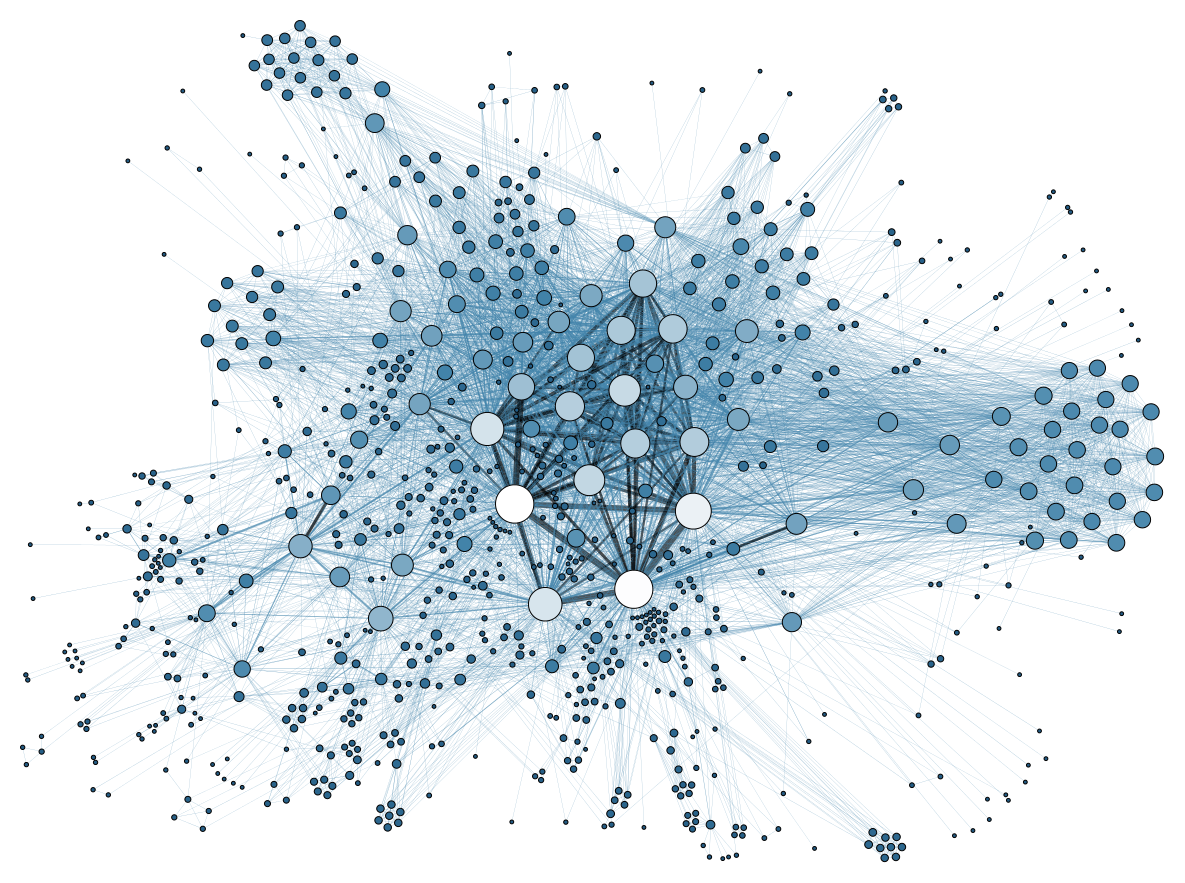
\includegraphics[width=0.75\textwidth]{praes_inginform_rot/Social_Network_Analysis_Visualization.png}
    \caption{\tiny{Quelle: $https://de.wikipedia.org/wiki/Soziale_Netzwerkanalyse#/media/Datei:Social$\_$Network$\_$Analysis$\_$Visualization.png$ (Stand 08.06.2022)}}
    \label{fig:my_label}
\end{figure}

\vspace{0.5cm}

\end{frame}

\begin{frame}
  %\frametitle{Fragestellung}
\vspace{-2.6cm}
\vspace{3.0cm}
\begin{figure}
    \centering
    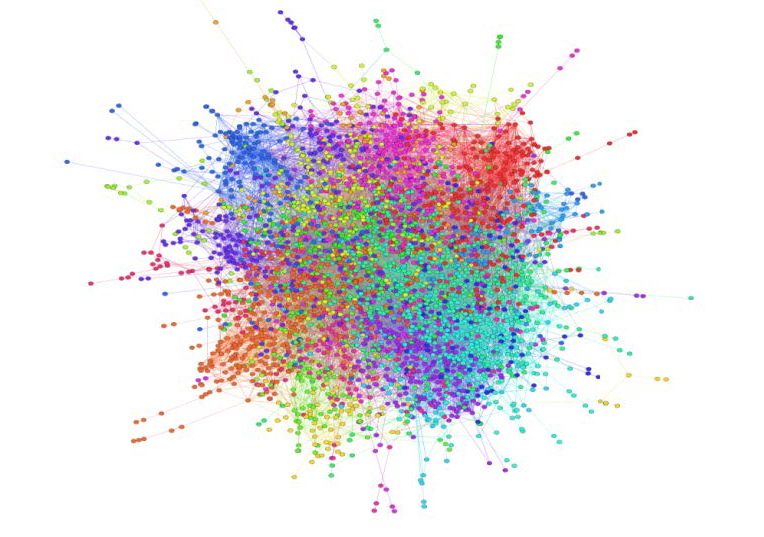
\includegraphics[width=0.75\textwidth]{praes_inginform_rot/network.png}
    \caption{\tiny{Quelle: $https://finetwork.wordpress.com/2015/05/26/free-workshop-on-social-network-analysis-sna/$ (Stand 08.06.2022)}}
    \label{fig:my_label}
\end{figure}

\vspace{0.5cm}

\end{frame}

\begin{frame}
  %\frametitle{Fragestellung}
\vspace{-2.6cm}
\vspace{3.0cm}
\begin{figure}
    \centering
    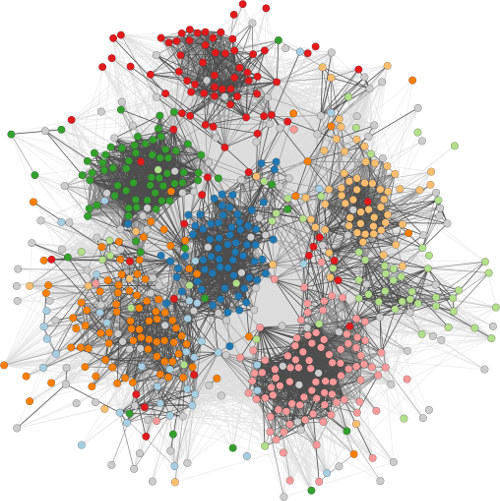
\includegraphics[width=0.55\textwidth]{praes_inginform_rot/lostCircles.jpg}
    \caption{\tiny{Quelle: $https://www.reddit.com/r/visualization/comments/439f91/visualize$\_$your$\_$facebook$\_$network/$ (Stand 08.06.2022)}}
    \label{fig:my_label}
\end{figure}

\vspace{0.5cm}

\end{frame}

\begin{frame}
  \frametitle{Gemeinsamkeiten und Kriterien}
\vspace{-2.6cm}
\vspace{2.0cm}
\begin{itemize}
    \item Cluster
    \item Brücken
    \item Cliquen
    \item Grad-Zentralität:
    $k_i &= \sum_{j=1}^{N} A_i_j$
    \item Nähe-Zentralität:
    $C_i &= \frac{N}{\sum_{j=1, j \not{=}i}^{N} d_i_j }$
    \item Zwischen-Zentralität:
    $B_i &= \sum_{(a-b)}\frac{\eta(a,i,b)}{\eta(a,b)}$
    \item Eigenvektor-Zentralität:
    $ c(v_i) = \sum_{j=1}^{N}a_{ij}c(v_j)$

\end{itemize}

\vspace{0.5cm}

\end{frame}


% 2. Folie
\section{Problematiken}
\begin{frame}
\vspace{-2.6cm}
\vspace{2.5cm}
  \frametitle{Problematiken}
  \begin{figure}
  \hspace{-2.5cm}
    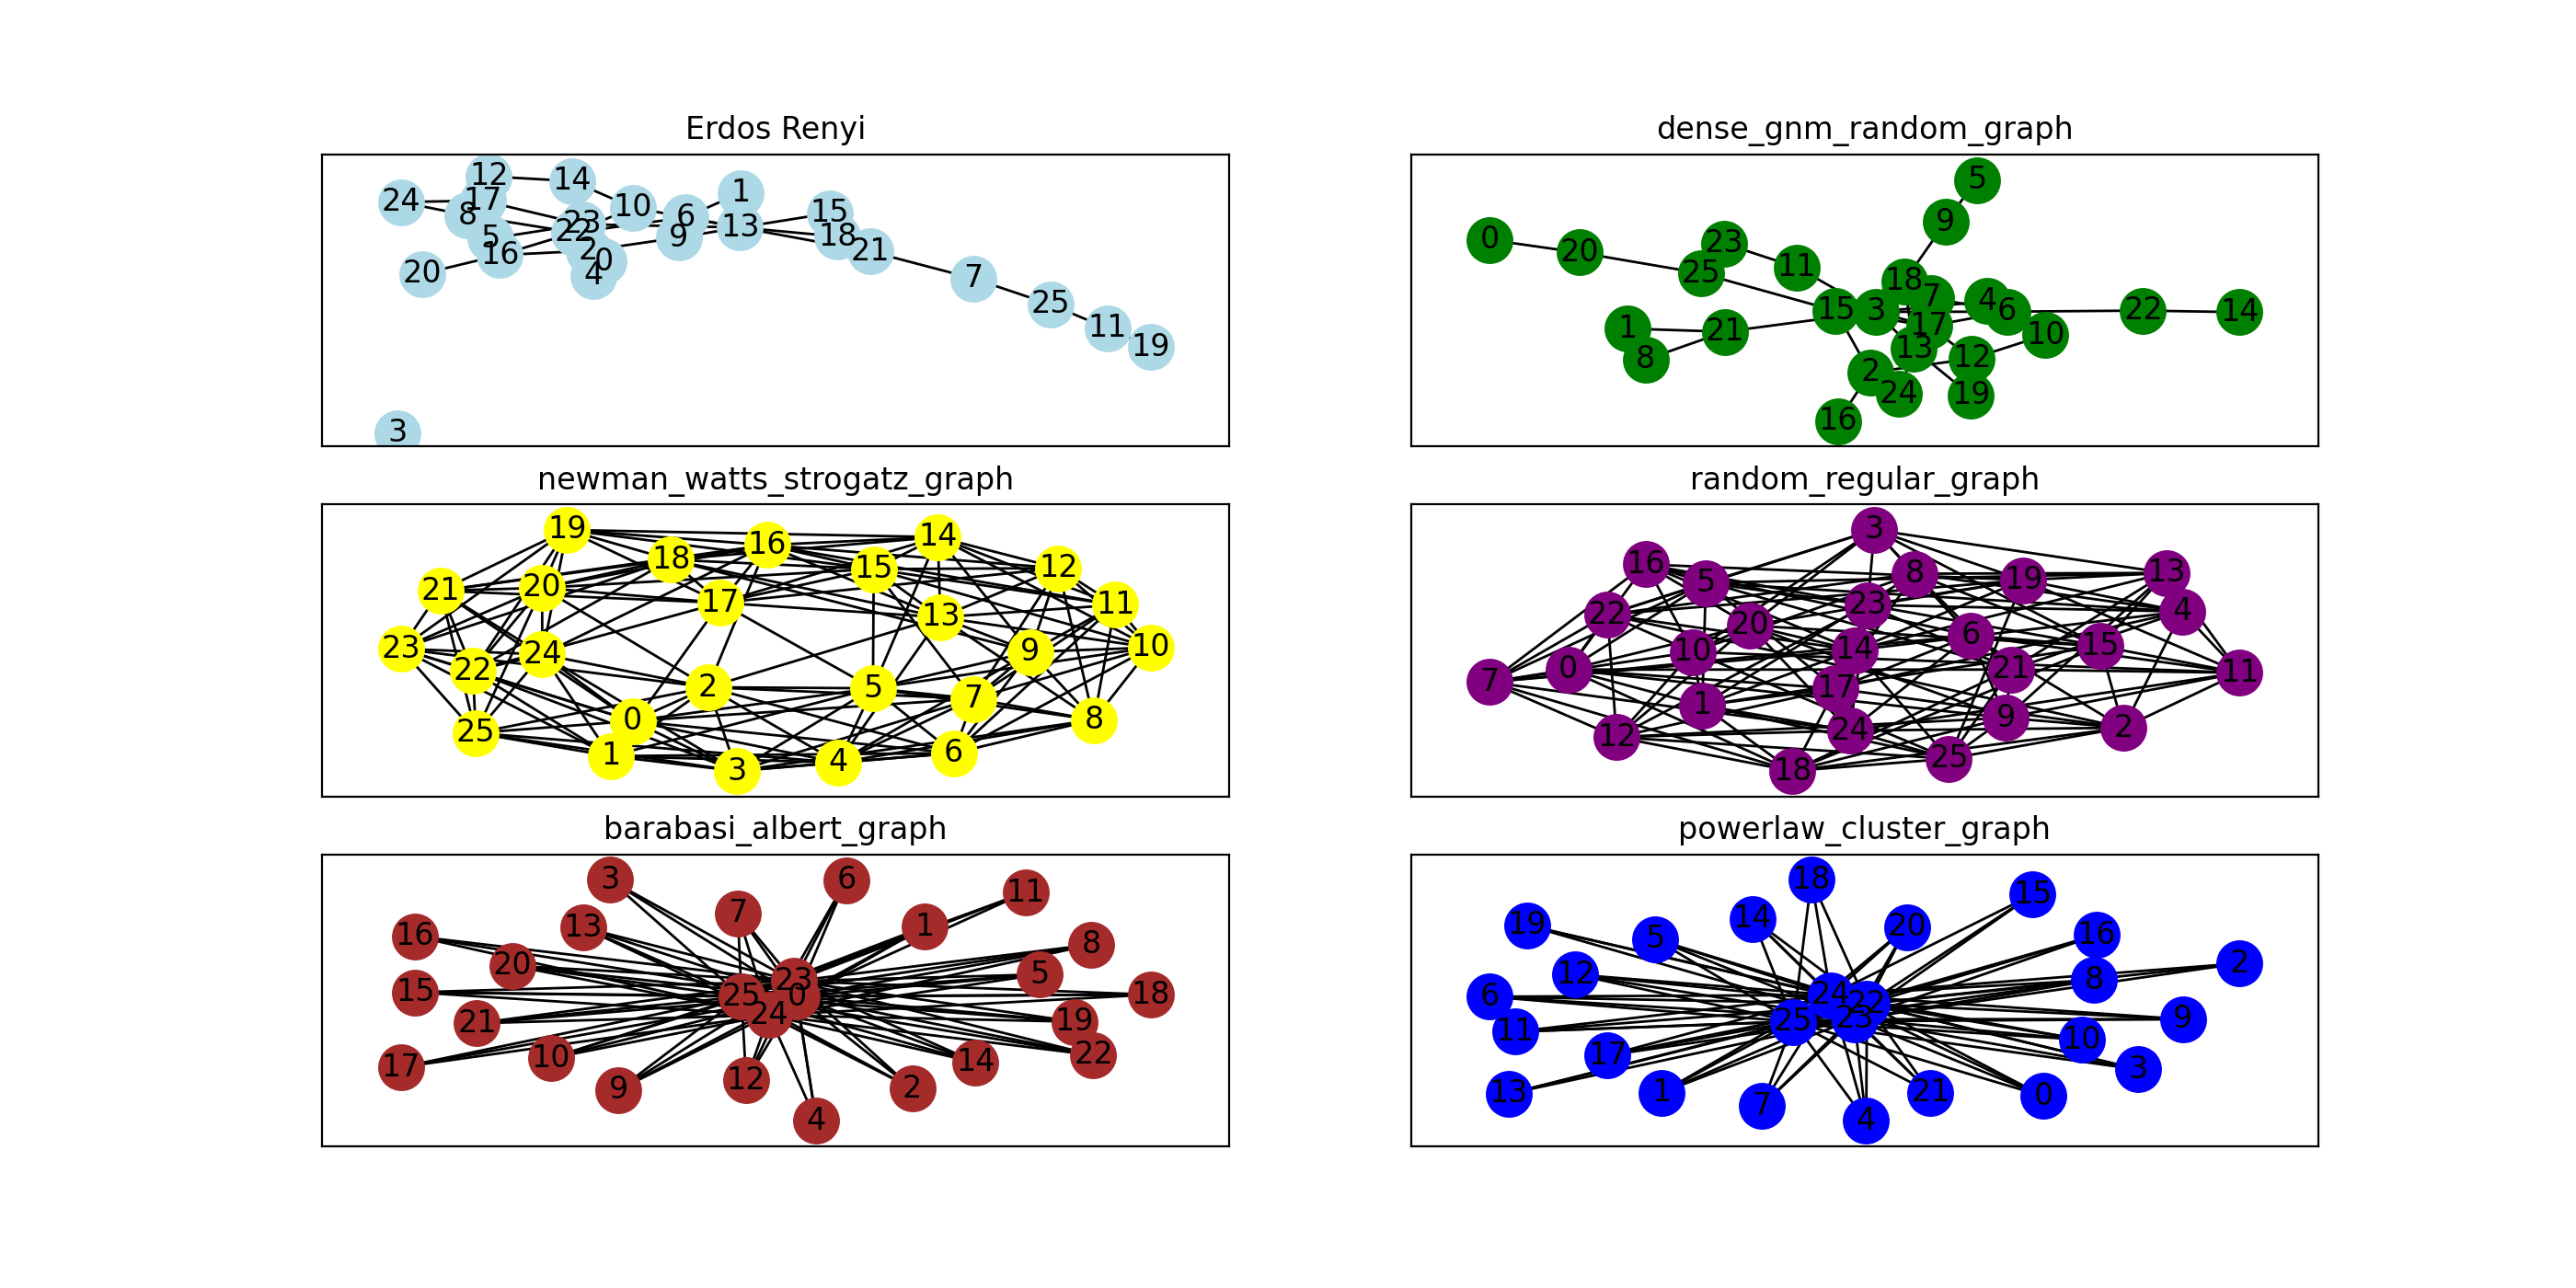
\includegraphics[width=1.25\textwidth]{praes_inginform_rot/6Random.png}
    \caption{\tiny{Quelle: Bachelor-Arbeit (Stand 08.06.2022)}}
    \label{fig:my_label}
\end{figure}
 
\end{frame}

% 3. Folie
\section{Implementierung}
\begin{frame}
  \frametitle{Implementierung}
\vspace{-2.6cm}
\vspace{2.0cm}
  \begin{figure}
  \centering
    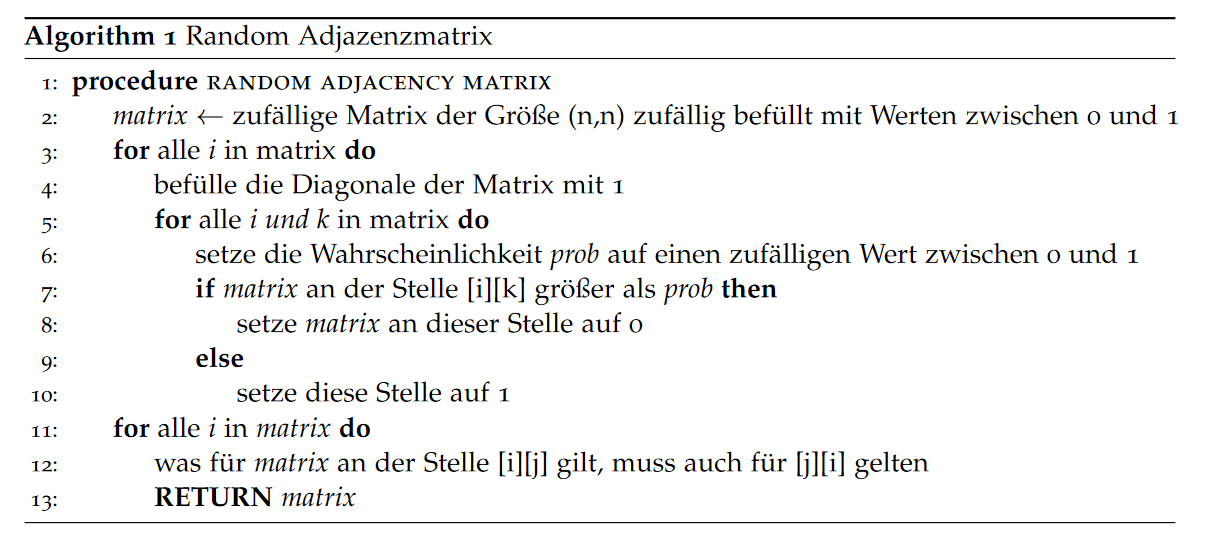
\includegraphics[width=1.0\textwidth]{praes_inginform_rot/Algo1.PNG}
    \caption{\tiny{Quelle: Bachelor-Arbeit (Stand 08.06.2022)}}
    \label{fig:my_label}
\end{figure}
\end{frame}

\begin{frame}
 %\frametitle{Implementierung}
\vspace{-2.6cm}
\vspace{2.0cm}
  \begin{figure}
  \centering
    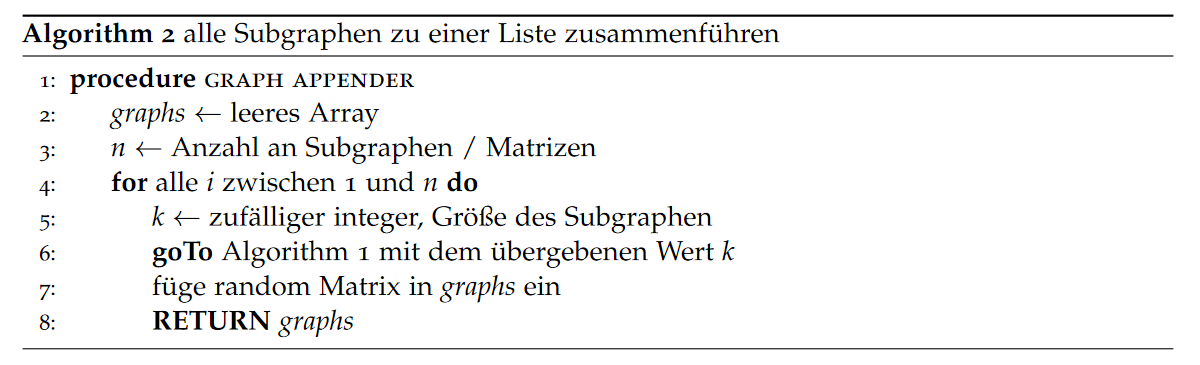
\includegraphics[width=1.0\textwidth]{praes_inginform_rot/Algo2.PNG}
    \caption{\tiny{Quelle: Bachelor-Arbeit (Stand 08.06.2022)}}
    \label{fig:my_label}
\end{figure}
\end{frame}

\begin{frame}
 %\frametitle{Implementierung}
\vspace{-2.6cm}
\vspace{2.0cm}
  \begin{figure}
  \centering
    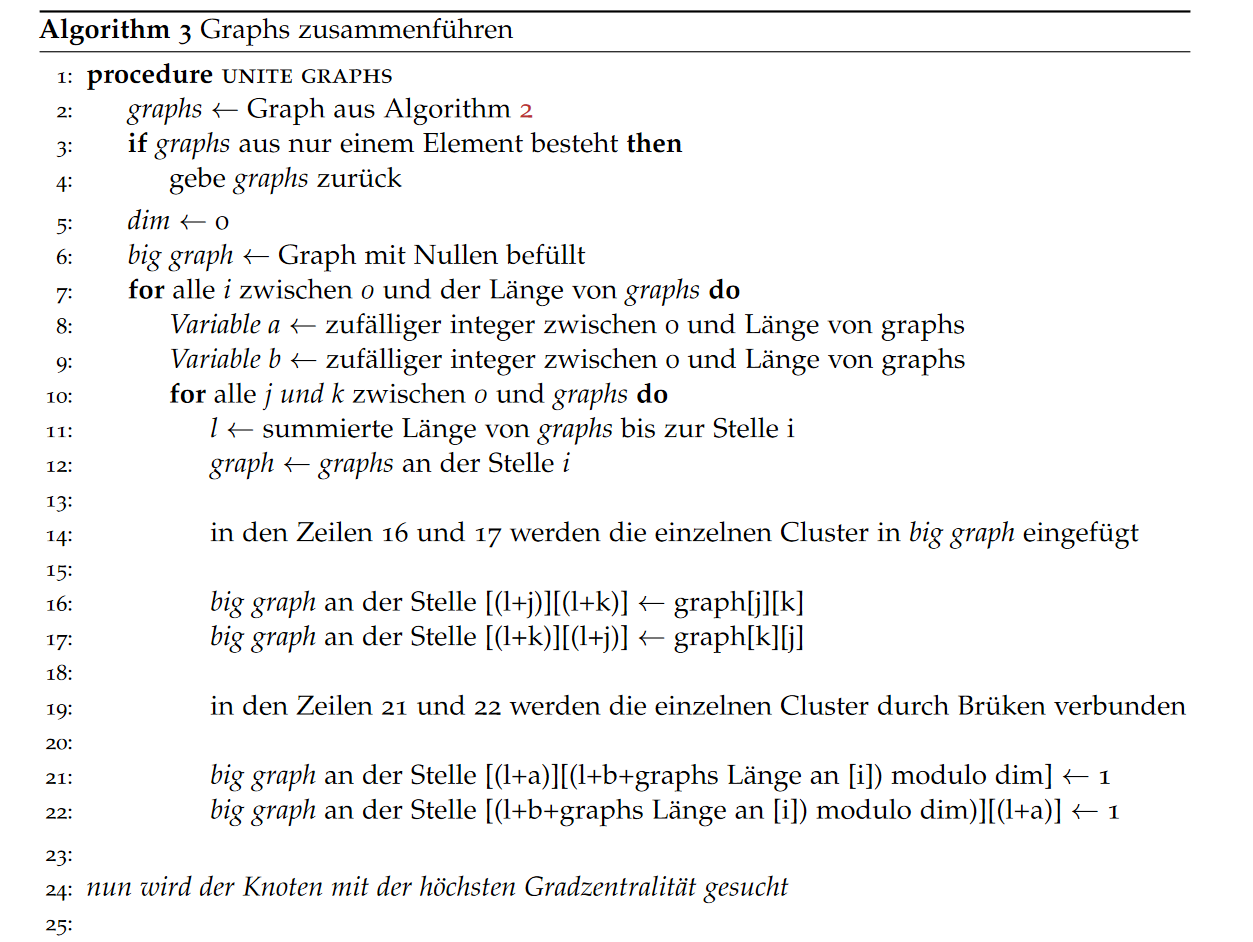
\includegraphics[width=1.0\textwidth]{praes_inginform_rot/Algo3.PNG}
    \caption{\tiny{Quelle: Bachelor-Arbeit (Stand 08.06.2022)}}
    \label{fig:my_label}
\end{figure}
\end{frame}

\begin{frame}
 %\frametitle{Implementierung}
\vspace{-2.6cm}
\vspace{2.0cm}
  \begin{figure}
  \centering
    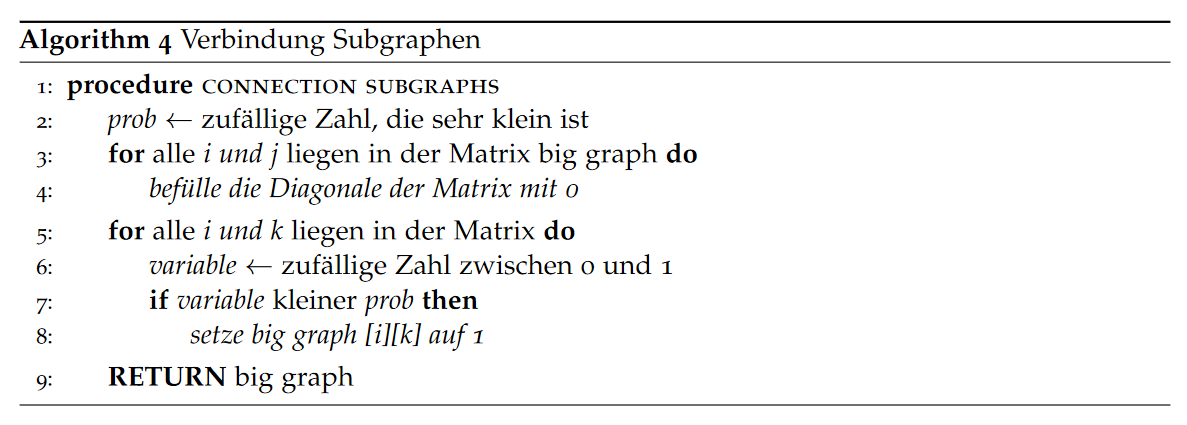
\includegraphics[width=1.0\textwidth]{praes_inginform_rot/Algo4.PNG}
    \caption{\tiny{Quelle: Bachelor-Arbeit (Stand 08.06.2022)}}
    \label{fig:my_label}
\end{figure}
\end{frame}
% 4. Folie


\section{Verteilung der Zentralitäten und Analyse}
\begin{frame}
  \frametitle{Verteilung der Zentralitäten und Analyse}
  \begin{figure}
  \centering
  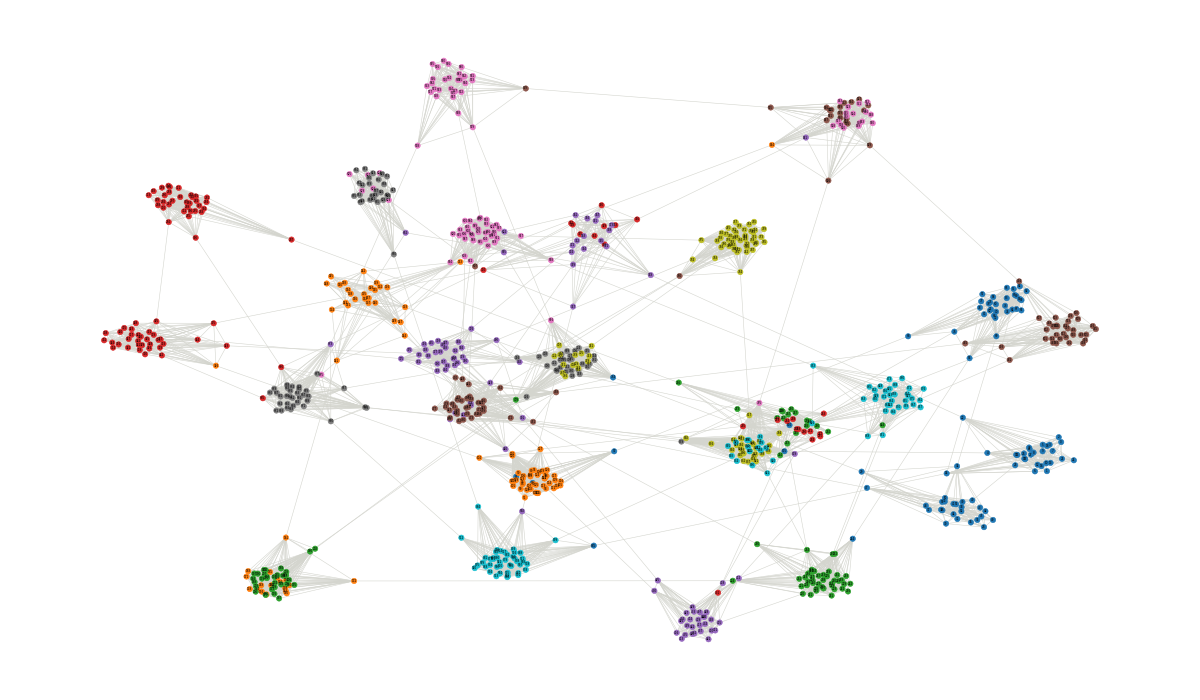
\includegraphics[width=0.5\textwidth]{praes_inginform_rot/newourSN.png}
  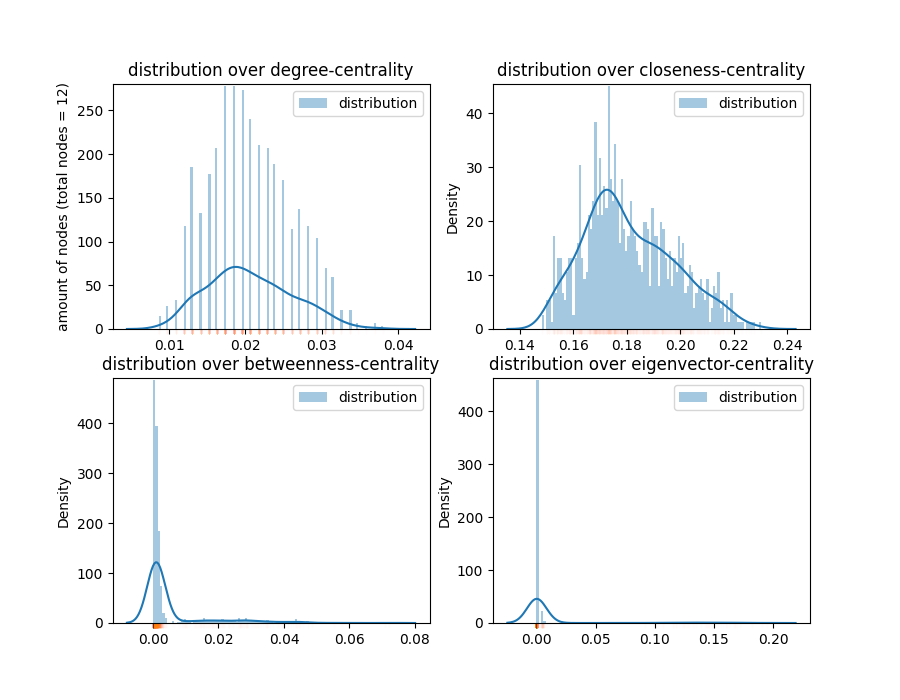
\includegraphics[width=0.45\textwidth]{praes_inginform_rot/newOurDist.png}
  \caption{Zufälliges soziales Netzwerk und Verteilungen(Quelle: Bachelor-Arbeit)}
  \label{fig:distributionALL}
\end{figure}
  

\end{frame}

% 5. Folie
\section{Ausblick / Optimierung}
\begin{frame}
  \frametitle{Ausblick / Optimierung}
\begin{itemize}
    \item Vergleich zu weiteren sozialen Netzwerken
    \item Optimierungen im Code
    \item Verteilungen genauer analysieren
    \item weitere Eigenschaften untersuchen

\end{itemize}
\vspace{-2.6cm}
\vspace{2.0cm}
\end{frame}


\section{Fazit und Fragen}
\begin{frame}
  \frametitle{Fazit und Fragen}
\vspace{-2.6cm}
\vspace{2.5cm}
  \begin{figure}
  \hspace{4cm}
  
\includegraphics[width=1.0\textwidth]{praes_inginform_rot/End.jpg}
 % \caption{Quelle: Bachelor-Arbeit}
  \label{fig:distributionALL}
\end{figure}

\end{frame}

\begin{frame}
  \frametitle{Poisson Verteilung: $P_\lambda(k)= \frac{\lambda^k}{k!}*e^-^\lambda$}
\vspace{-2.6cm}
\vspace{2.5cm}
  \begin{figure}
  \hspace{4cm}
  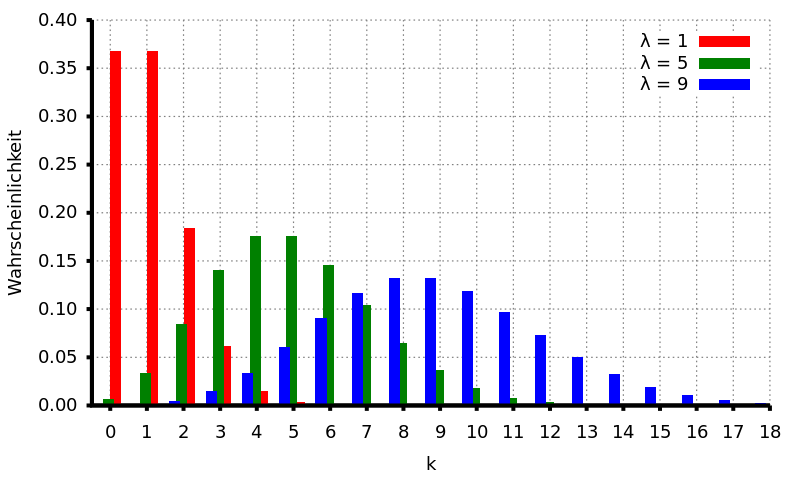
\includegraphics[width=1.0\textwidth]{praes_inginform_rot/Poisson-Verteilung.png}
  \caption{Quelle: $https://de.wikipedia.org/wiki/Poisson-Verteilung#/media/Datei:Poisson-Verteilung$\_$1$\_$5$\_$9.svg$}
  \label{fig:distributionALL}
\end{figure}
\end{frame}

\begin{frame}
  \frametitle{Facebook Netzwerk}
\vspace{-2.6cm}
\vspace{2.5cm}
  \begin{figure}
  \hspace{4cm}
  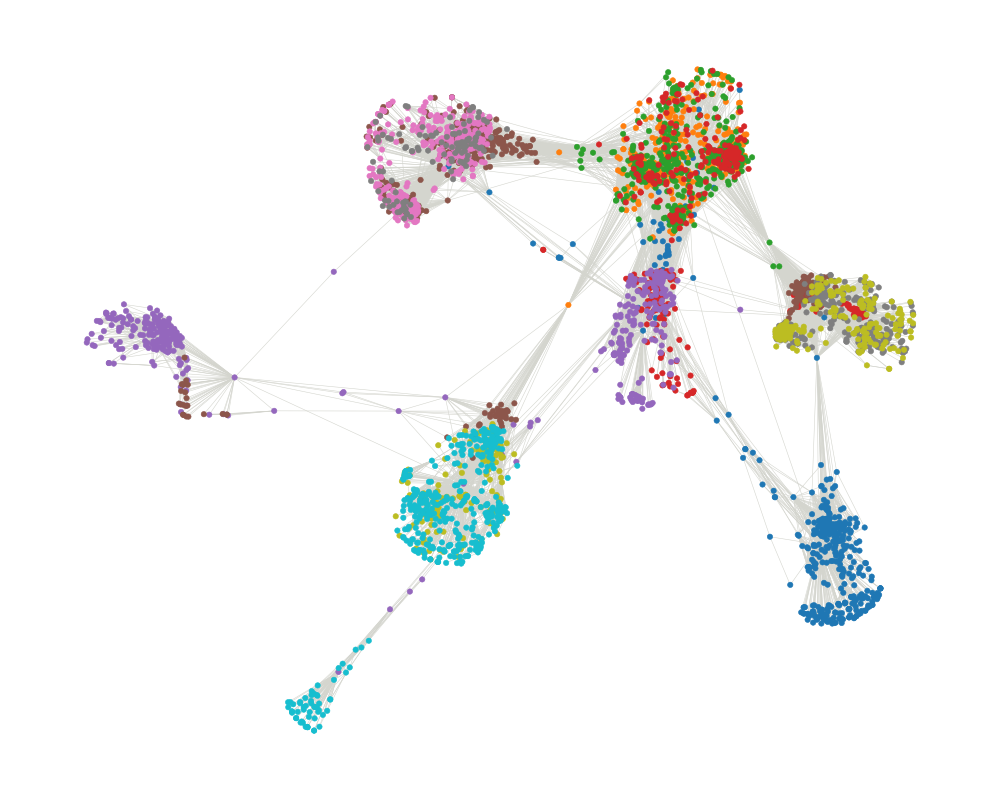
\includegraphics[width=0.75\textwidth]{praes_inginform_rot/FacebookPlot.png}
  \caption{Quelle: Bachelor-Arbeit}
  \label{fig:distributionALL}
\end{figure}
\end{frame}

\begin{frame}
  %\frametitle{Bestehende soziale Netzwerke}
\vspace{-2.6cm}
\vspace{2.5cm}
  \begin{figure}
  \hspace{4cm}
  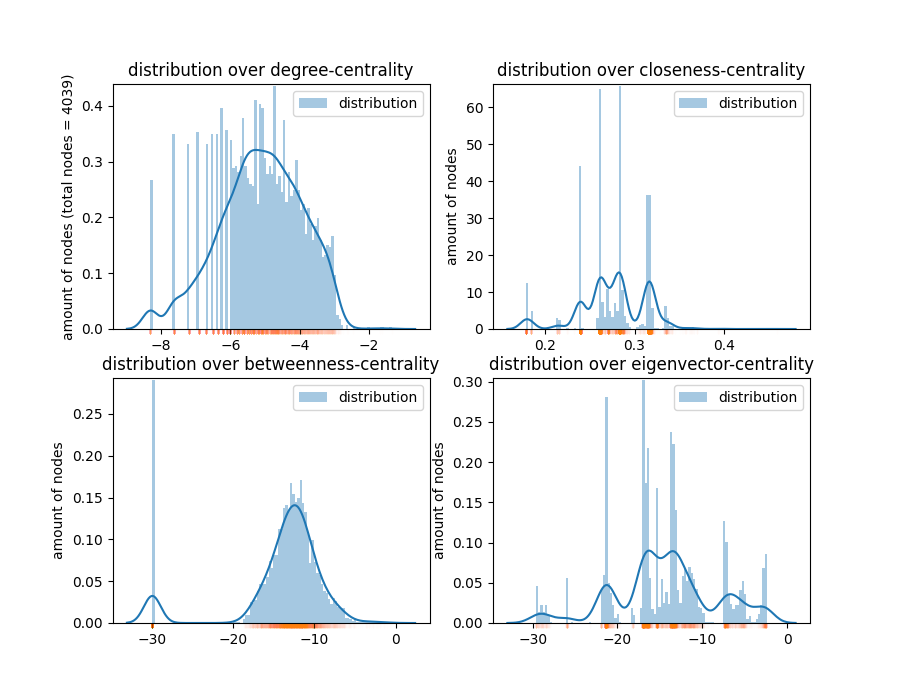
\includegraphics[width=0.75\textwidth]{praes_inginform_rot/FB-Distribution.png}
  \caption{Quelle: Bachelor-Arbeit}
  \label{fig:distributionALL}
\end{figure}
\end{frame}

\begin{frame}
  \frametitle{Game Of Thrones Netzwerk}
\vspace{-2.6cm}
\vspace{2.5cm}
  \begin{figure}
  \hspace{4cm}
  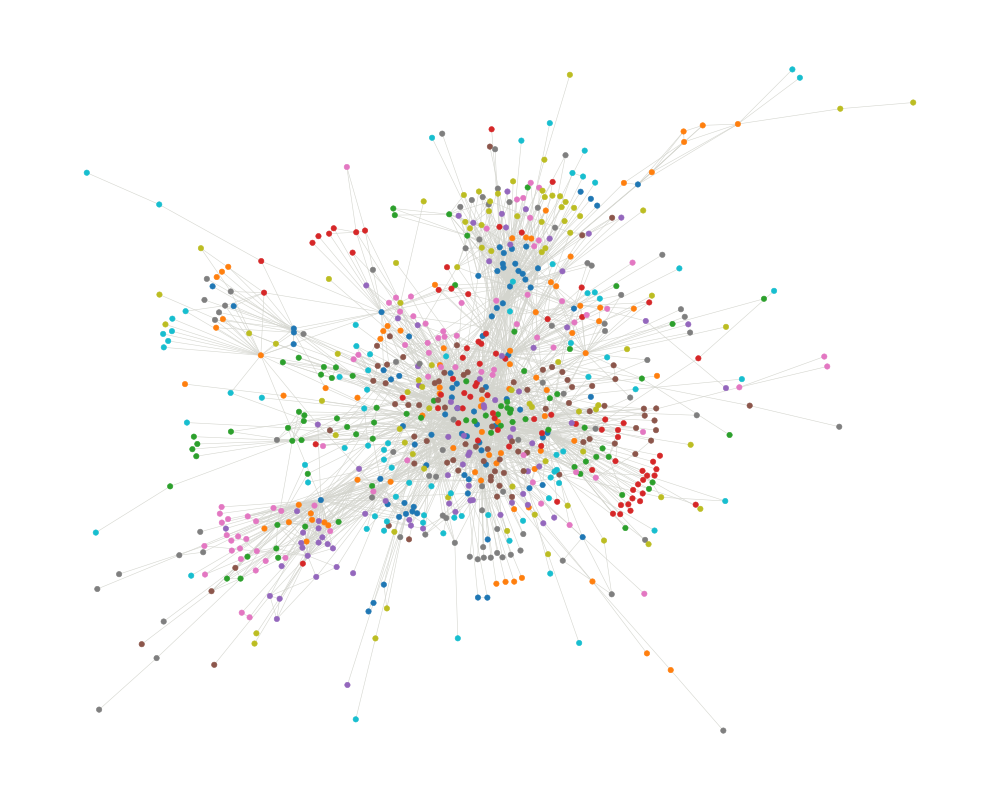
\includegraphics[width=0.75\textwidth]{praes_inginform_rot/GOT-Plot.png}
  \caption{Quelle: Bachelor-Arbeit}
  \label{fig:distributionALL}
\end{figure}
\end{frame}

\begin{frame}
  %\frametitle{Bestehende soziale Netzwerke}
\vspace{-2.6cm}
\vspace{2.5cm}
  \begin{figure}
  \hspace{4cm}
  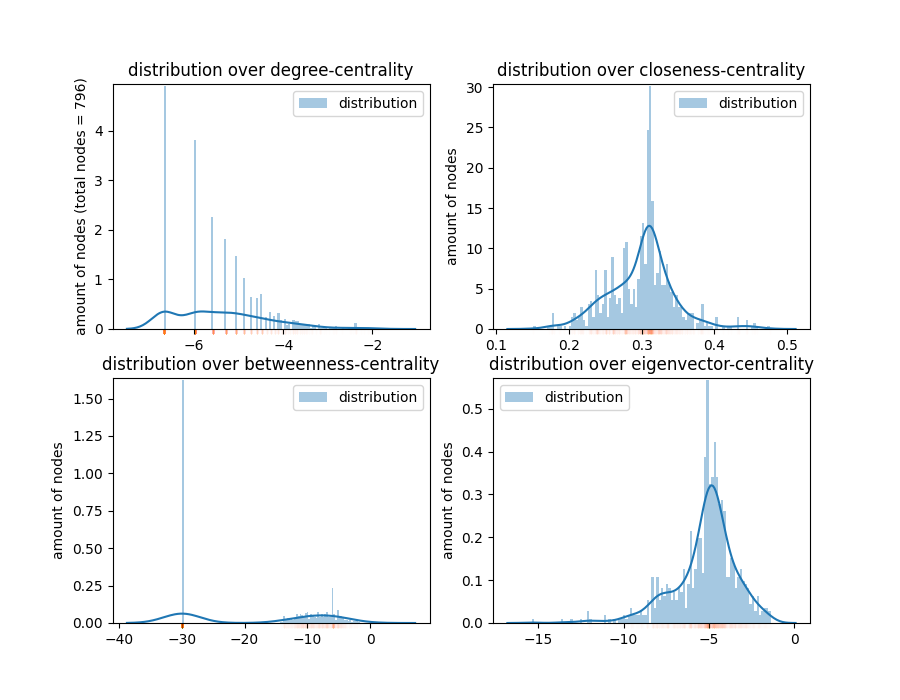
\includegraphics[width=0.75\textwidth]{praes_inginform_rot/GOT-Distribution.png}
  \caption{Quelle: Bachelor-Arbeit}
  \label{fig:distributionALL}
\end{figure}
\end{frame}

\begin{frame}
  \frametitle{Selbst generiertes Netzwerk}
\vspace{-2.6cm}
\vspace{2.5cm}
  \begin{figure}
  \hspace{4cm}
  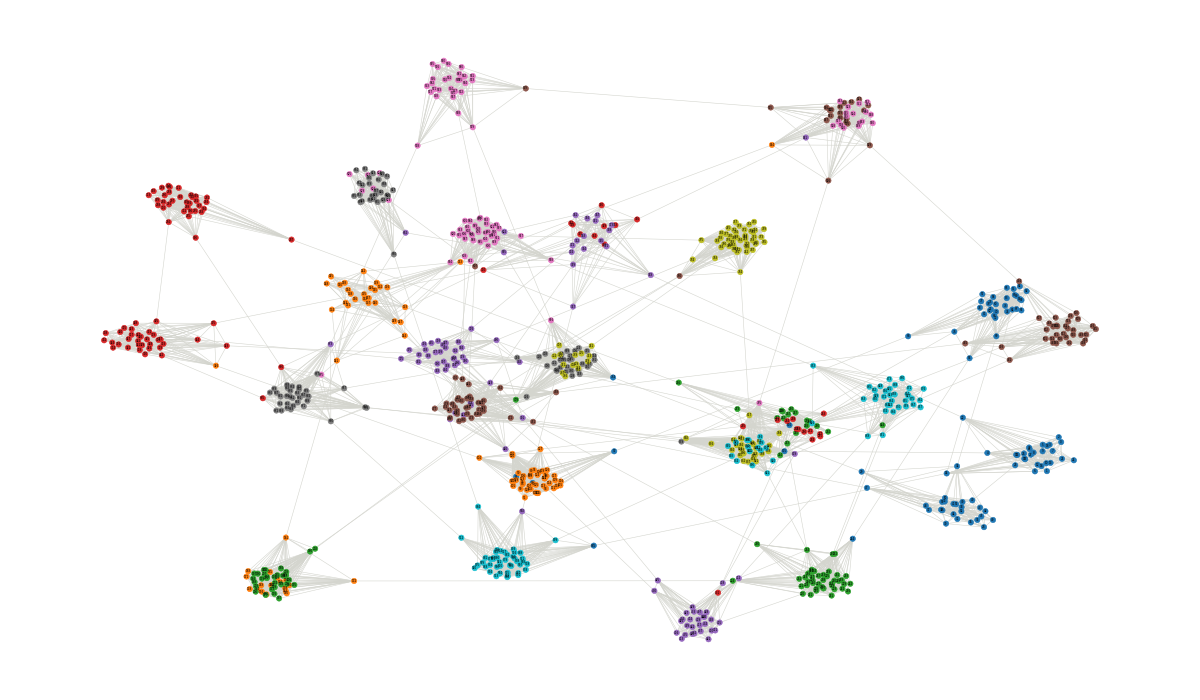
\includegraphics[width=0.75\textwidth]{praes_inginform_rot/newourSN.png}
  \caption{Quelle: Bachelor-Arbeit}
  \label{fig:distributionALL}
\end{figure}
\end{frame}

\begin{frame}
  %\frametitle{Bestehende soziale Netzwerke}
\vspace{-2.6cm}
\vspace{2.5cm}
  \begin{figure}
  \hspace{4cm}
  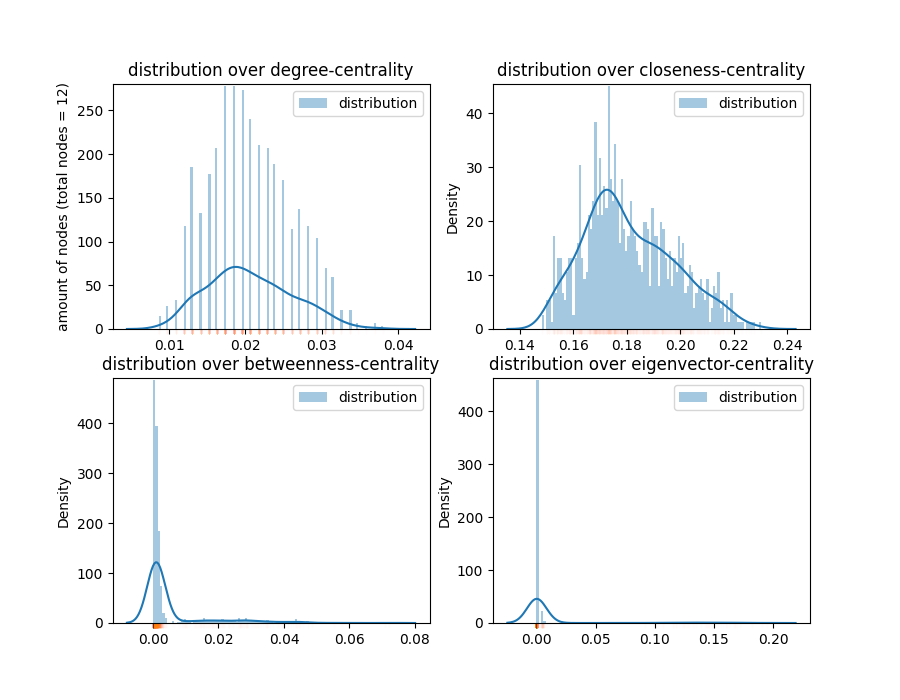
\includegraphics[width=0.75\textwidth]{praes_inginform_rot/newOurDist.png}
  \caption{Quelle: Bachelor-Arbeit}
  \label{fig:distributionALL}
\end{figure}
\end{frame}

\end{document}